\documentclass[a4paper, 11pt]{article}           %{{{1
% basic packages                                  {{{2
\usepackage[T1]{fontenc}
\usepackage[scaled=0.975]{helvet}
\usepackage[utf8]{inputenc}
\usepackage{amsmath}
\usepackage{lastpage}
\usepackage{graphicx}
\usepackage{amsfonts}
\usepackage{variations}
\usepackage{pgf,tikz}           % dessin
\usepackage{mathrsfs}
\usetikzlibrary{arrows}
\usepackage{pgfkeys}        % fenetrage des plot TikZ
\usepackage{yhmath}         % arc au dessus des lettres
\usepackage{calc}           % calcul de longueur
\usepackage{variations}     % tableau de variations
\usepackage{multicol}
\usepackage{enumitem}
%\usepackage{listings}       % syntax highlightingn of most common languages
%\usepackage{color}
%}}}

% mise en page                                    {{{2
\addtolength{\voffset}{-1.8cm}
\addtolength{\textheight}{4cm}
\addtolength{\hoffset}{-2.5cm}
\addtolength{\textwidth}{4cm}
\addtolength{\headsep}{-0.5cm}
\usepackage{fancyhdr}
\setlength{\headheight}{14.00pt}
\pagestyle{fancy} % Numérotation des pages
\renewcommand\headrulewidth{1pt}
\fancyhead[L]{2nd SN}
\fancyhead[C]{Système de sécurité incendie}
\fancyhead[R]{\textbf{Habitat intelligent}}
\renewcommand\footrulewidth{1pt}
\fancyfoot[L]{v 1.0 - non testé}
\fancyfoot[C]{octobre 2017}
\fancyfoot[R]{\thepage/\pageref{LastPage}}
%\lhead{3E}%haut de page gauche
%}}}

% Compteurs:                                     {{{2
\addtocounter{page}{0}
\newcounter{Q}
\newcounter{exoNB}
%}}}

% Longueur:                                      {{{2
\newlength{\longueurA}
\newlength{\longueurB}
\setlength{\parindent}{0pt}
\setlength{\parskip}{2pt}
\renewcommand{\baselinestretch}{1}
%}}}

% Divers                                          {{{2
% listings                                        {{{3
%\definecolor{mygreen}{rgb}{0,0.6,0}
%\definecolor{mygray}{rgb}{0.5,0.5,0.5}
%\definecolor{mymauve}{rgb}{0.58,0,0.82}
%\definecolor{deepblue}{rgb}{0,0,0.5}
%\definecolor{deepred}{rgb}{0.6,0,0}
%\definecolor{deepgreen}{rgb}{0,0.5,0}
%\lstset{%
%        backgroundcolor=\color{white},   % choose the background color; you must add \usepackage{color} or \usepackage{xcolor}; should come as last argument
%        basicstyle=\footnotesize,        % the size of the fonts that are used for the code
%        breakatwhitespace=false,         % sets if automatic breaks should only happen at whitespace
%        breaklines=true,                 % sets automatic line breaking
%        captionpos=b,                    % sets the caption-position to bottom
%        commentstyle=\color{mygreen},    % comment style
%        deletekeywords={...},            % if you want to delete keywords from the given language
%        escapeinside={\%*}{*)},          % if you want to add LaTeX within your code
%        extendedchars=true,              % lets you use non-ASCII characters; for 8-bits encodings only, does not work with UTF-8
%        frame=single,                    % adds a frame around the code
%        keepspaces=true,                 % keeps spaces in text, useful for keeping indentation of code (possibly needs columns=flexible)
%        keywordstyle=\color{blue},       % keyword style
%        morekeywords={*,...},            % if you want to add more keywords to the set
%        numbers=left,                    % where to put the line-numbers; possible values are (none, left, right)
%        numbersep=5pt,                   % how far the line-numbers are from the code
%        numberstyle=\tiny\color{mygray}, % the style that is used for the line-numbers
%        rulecolor=\color{black},         % if not set, the frame-color may be changed on line-breaks within not-black text (e.g. comments (green here))
%        showspaces=false,                % show spaces everywhere adding particular underscores; it overrides 'showstringspaces'
%        showstringspaces=false,          % underline spaces within strings only
%        showtabs=false,                  % show tabs within strings adding particular underscores
%        stepnumber=2,                    % the step between two line-numbers. If it's 1, each line will be numbered
%        stringstyle=\color{mymauve},     % string literal style
%        tabsize=4,                       % sets default tabsize to 2 spaces
%        title=\lstname                   % show the filename of files included with \lstinputlisting; also try caption instead of title
%}
%\lstset{%
%        language=Python,                 % the language of the code
%        otherkeywords={self},            % Add keywords here
%        deletekeywords={type},           % if you want to delete keywords from the given language
%        emph={},                         % Custom highlighting
%        emphstyle=\ttb\color{deepred}    % Custom highlighting style
%}
%}}}

% PRL style line                                 {{{3
\newlength{\diamondrulelength}
\setlength{\diamondrulelength}{0.6\textwidth}
\newlength{\diamondrulethickness}
\setlength{\diamondrulethickness}{2pt}
\newcommand{\diamondrule}{\begin{center}\tikz{\fill[black] (0.5\diamondrulelength,0) -- (0,0.5\diamondrulethickness) -- (-0.5\diamondrulelength,0) -- (0,-0.5\diamondrulethickness) -- cycle;}\end{center}}
%}}}

% fixed with tabular                             {{{3
\usepackage{array}
\newcolumntype{L}[1]{>{\raggedright\let\newline\\\arraybackslash\hspace{0pt}}m{#1}}
\newcolumntype{C}[1]{>{\centering\let\newline\\\arraybackslash\hspace{0pt}}m{#1}}
\newcolumntype{R}[1]{>{\raggedleft\let\newline\\\arraybackslash\hspace{0pt}}m{#1}}
%}}}

%}}}
%}}}

\begin{document}
\sffamily

% https://www.instructables.com/id/Arduino-Modules-Flame-Sensor/
% $2.60 dx.com SKU = 389613

\begin{center}
\textsc{Système d'alarme}\\
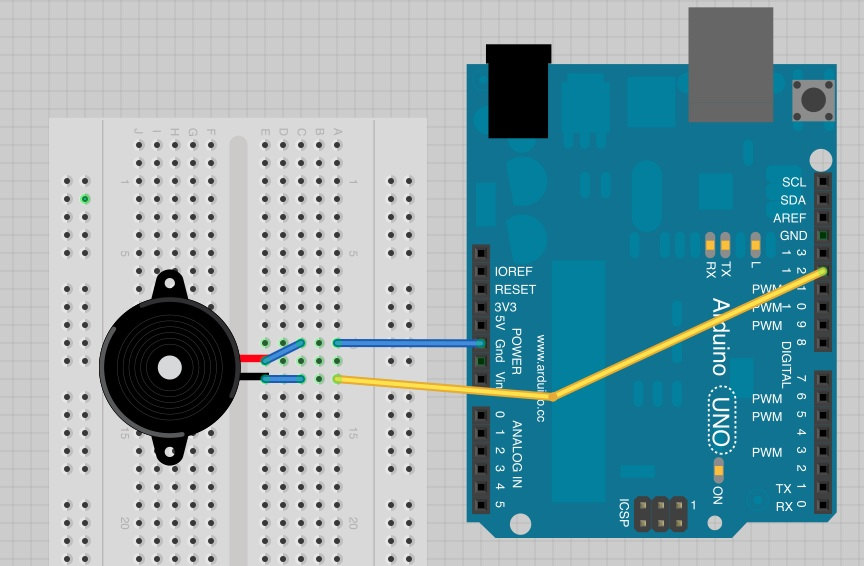
\includegraphics[width=0.6\textwidth]{learn_arduino_fritzing}
\end{center}


\stepcounter{Q}$\boxed{\arabic{Q}}$ Qu'est ce qu'un matériau piezzo-électrique?\\
\underline{\hspace{\textwidth}} \\[0.2cm]

\stepcounter{Q}$\boxed{\arabic{Q}}$ Donner un example de capteur utilisant un tel matériau.\\
\underline{\hspace{\textwidth}} \\[0.2cm]

\stepcounter{Q}$\boxed{\arabic{Q}}$ Donner un example d'actionneur utilisant un tel matériau.\\
\underline{\hspace{\textwidth}} \\[0.2cm]

\begin{center}
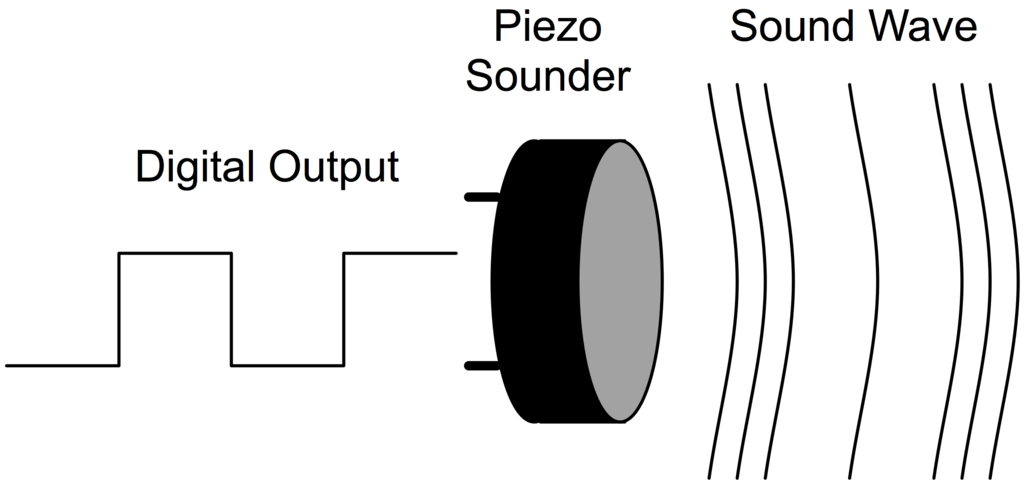
\includegraphics[width=0.5\textwidth]{sound_process}
\end{center}
\stepcounter{Q}$\boxed{\arabic{Q}}$ Que sont les ondes sonores ? \\
\underline{\hspace{\textwidth}} \\[0.2cm]

\stepcounter{Q}$\boxed{\arabic{Q}}$ Quelle est la fréquence du LA donné par le diapason conventionnel ? \\
\underline{\hspace{\textwidth}} \\[0.2cm]




\textsc{Réalisation d'une gamme}\\

\stepcounter{Q}$\boxed{\arabic{Q}}$ A l'aide du code suivant, réaliser une gamme. \\
\scriptsize %{{{1
\begin{verbatim}
int speakerPin = 12;

int numTones = 10;
int tones[] = {261, 277, 294, 311, 330, 349, 370, 392, 415, 440};
//            mid C  C#   D    D#   E    F    F#   G    G#   A

void setup()
{
  for (int i = 0; i < numTones; i++)
  {
    tone(speakerPin, tones[i]);
    delay(500);
  }
  noTone(speakerPin);
}

void loop()
{
}
\end{verbatim} %}}}
\normalsize
Constation professeur :

\stepcounter{Q}$\boxed{\arabic{Q}}$ Que fait la boucle for ? \\
\underline{\hspace{\textwidth}} \\[0.2cm]

\stepcounter{Q}$\boxed{\arabic{Q}}$ Que fait la commande tone() ? \\
\underline{\hspace{\textwidth}} \\[0.2cm]


\textsc{Réalisation d'un pseudo thérémine}\\

\begin{center}
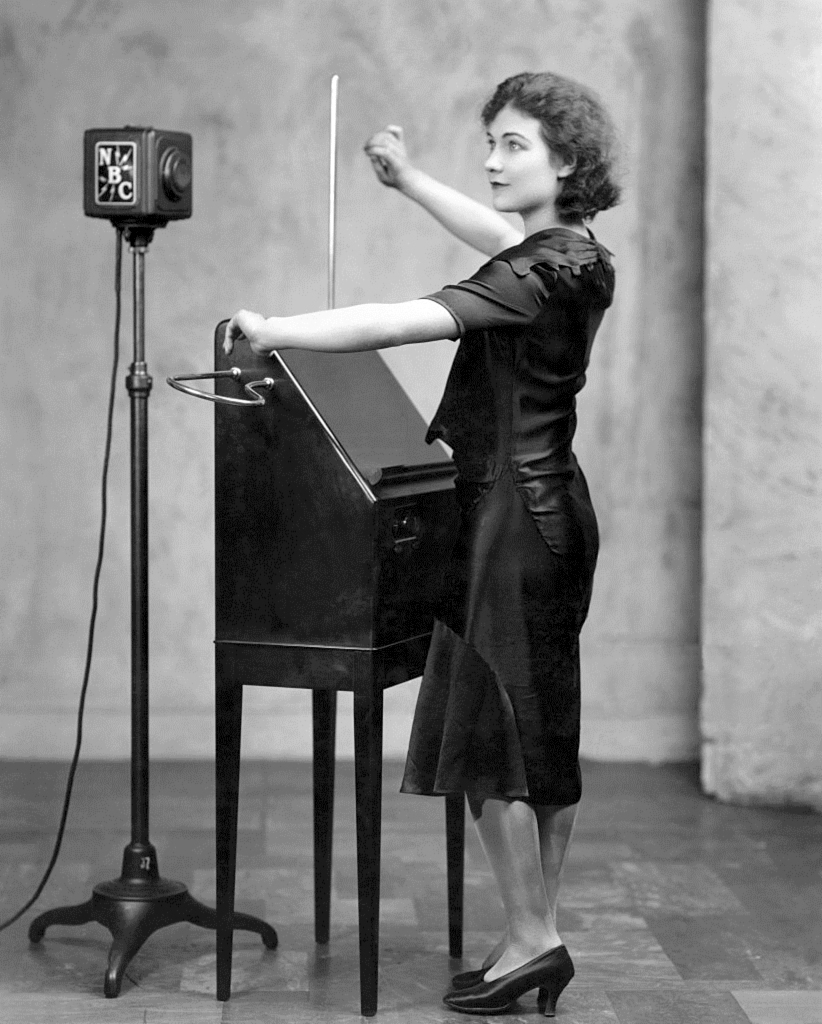
\includegraphics[width=0.3\textwidth]{Theramin-Alexandra-Stepanoff-1930}\\
Alexandra Stepanoff jouant au theremine à la radio NBC, 1930
\end{center}

\stepcounter{Q}$\boxed{\arabic{Q}}$ Quel est le principe d'un théremine ? Donner un morceau que vous connaissez où il est utilisé. \\
\underline{\hspace{\textwidth}} \\[0.2cm]

\begin{center}
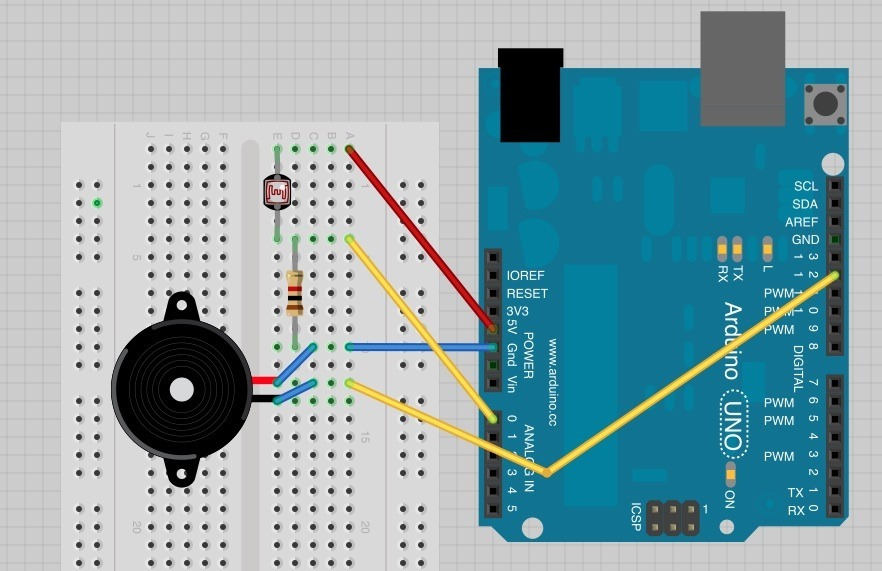
\includegraphics[width=0.5\textwidth]{theremine_cablage}\\
Pseudo-thérémine.
\end{center}
\stepcounter{Q}$\boxed{\arabic{Q}}$ Réaliser le cablage du pseudo-thérémine. \\
Constation du professeur :

\stepcounter{Q}$\boxed{\arabic{Q}}$ A l'aide du code suivant, réaliser un pseudo thérémine. \\
\scriptsize %{{{1
\begin{verbatim}
int speakerPin = 12;
int photocellPin = 0;

void setup()
{
}

void loop()
{
  int reading = analogRead(photocellPin);
  int pitch = 200 + reading / 4;
  tone(speakerPin, pitch);
}
\end{verbatim} %}}}
\normalsize

\stepcounter{Q}$\boxed{\arabic{Q}}$ Quel est la mesure physique stockée dans la variable reading ? \\
\underline{\hspace{\textwidth}} \\[0.2cm]

\stepcounter{Q}$\boxed{\arabic{Q}}$ Estimer l'intervalle de fréquences générées ? \\
\underline{\hspace{\textwidth}} \\[0.2cm]




\textsc{Réalisation d'une mélodie}\\
\begin{center}
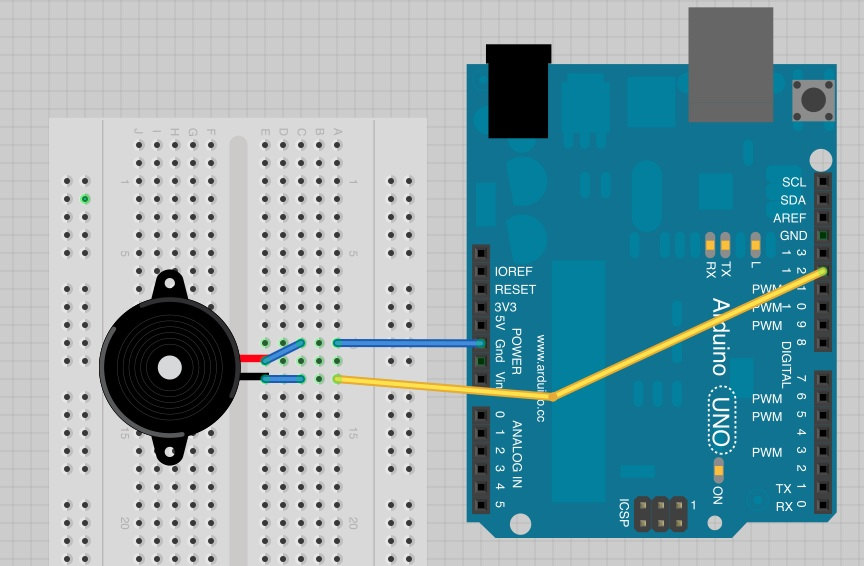
\includegraphics[width=0.4\textwidth]{learn_arduino_fritzing}
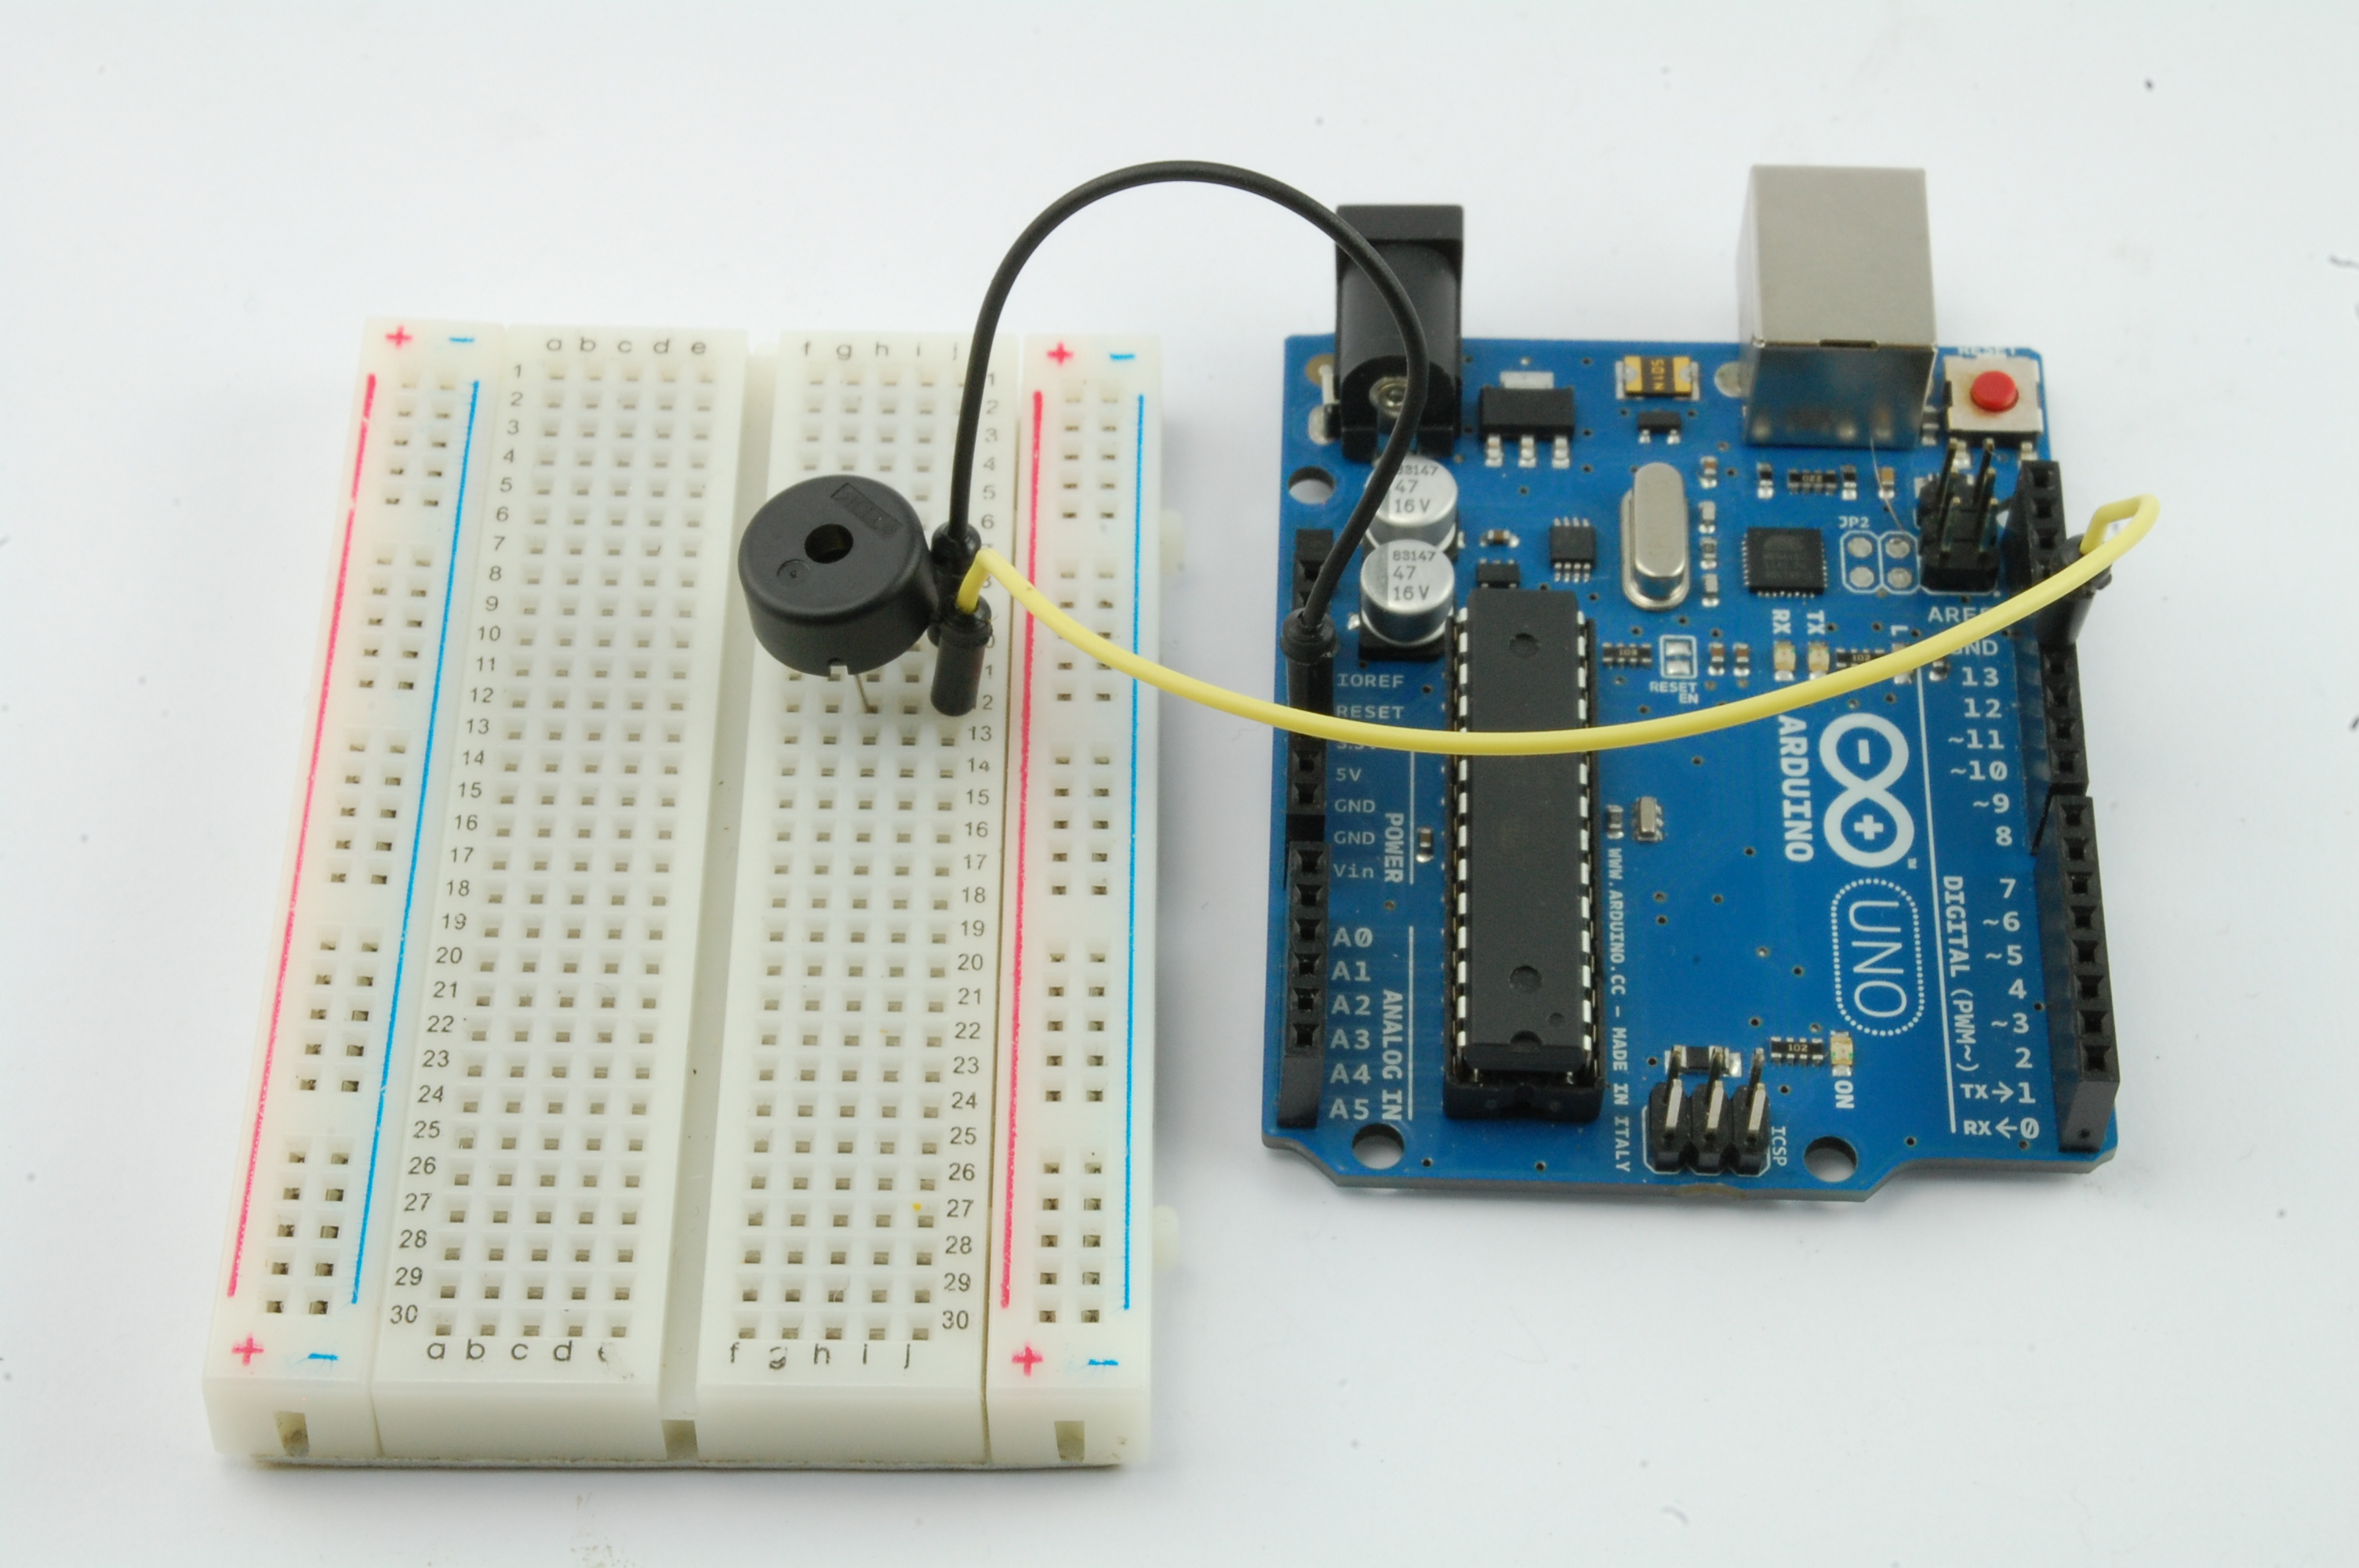
\includegraphics[width=0.4\textwidth]{learn_arduino_just_sounder}
\end{center}
Le code source du programme se trouve dans ce tutoriel : \\
{\tt https://www.princetronics.com/supermariothemesong/}

\stepcounter{Q}$\boxed{\arabic{Q}}$ Dans la source du programme, expliquez le role des commandes define (voir aussi lienmini.fr/e119-test).\\
\underline{\hspace{\textwidth}} \\[0.2cm]

\stepcounter{Q}$\boxed{\arabic{Q}}$ Faire constater au professeur que les thèmes de \emph{mario} et de \emph{underworkd} sont bien jouées.\\
Constation professeur :


\end{document}
%vim:fdm=marker



\end{document}
%vim:fdm=marker

